\documentclass[border=10pt]{standalone}
\usepackage{tikz}
\begin{document}
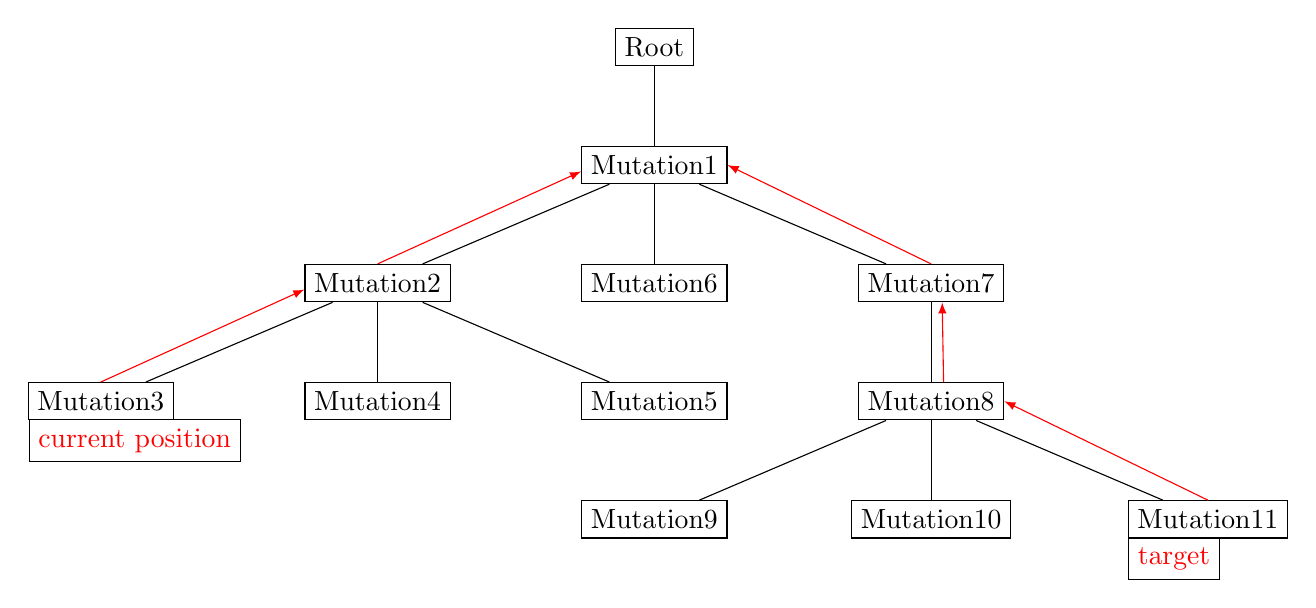
\begin{tikzpicture}[sibling distance=10em,
  every node/.style = {shape=rectangle, draw}]]
  	\node {Root}
    	child { node (Mutation1) {Mutation1} 
	  		child { node (Mutation2) {Mutation2}
        		child { node (Mutation3) {Mutation3} }
        		child { node {Mutation4} }
        		child { node {Mutation5} } }
      		child { node {Mutation6} } 
    		child { node (Mutation7) {Mutation7}
      			child { node (Mutation8) {Mutation8}
        			child { node {Mutation9} }
        			child { node {Mutation10} }
        			child { node (Mutation11) {Mutation11} } } } };
         
   	\node[text=red] at (-6.6,-5) {current position};
   	\node[text=red] at (6.6,-6.5) {target};  
   	   
   	\draw[-latex,red] (Mutation3.north) -- (Mutation2.185);
   	\draw[-latex,red] (Mutation2.north) -- (Mutation1.185);
   	\draw[-latex,red] (Mutation7.north) -- (Mutation1.east);
   	\draw[-latex,red] (Mutation8.57) -- (Mutation7.300);
   	\draw[-latex,red] (Mutation11.north) -- (Mutation8.east);
   	   		   	             
\end{tikzpicture}
\end{document}
